%!TEX root = ../main.tex

\chapter{Introduction}
\label{chp:intro}

\section{Case introduction}
\noindent
The pediatric cardiac surgery unit of the university hospital of Padova is an important center, handling more than 300\footnote{\url{https://www.aopd.veneto.it/Cardiochirurgia-Pediatrica}} cases per year. The center specializes in surgical treatment of simple and complex congenital heart disease, at any age.
The need to teach and visualize the case of operation is very important. \\
Thanks to \ac{MRI} and \ac{CT} scans, surgeons can not only view detailed images of the heart, but also create 3D models Fig.[\ref{fig:heart}], as explained in this thesis Bib.\cite{thesisFrancesco}. These images are essential for pre-operative planning and understanding the patient's condition.
In special cases, 3D models can further enhance understanding of patients with particularly complex heart problems.
3D models can also be used to create molds for producing silicone replicas, allowing surgeons to practice the procedure before performing it on the patient, as explained in Bib.\cite{thesisFabio}.
This approach is typically reserved for special cases, but it can be extremely valuable for future procedures and educational purposes.\\
The application discussed in this thesis will use these 3D models for only training purposes without any simulation.\\

\begin{figure}[ht]
  \centering
  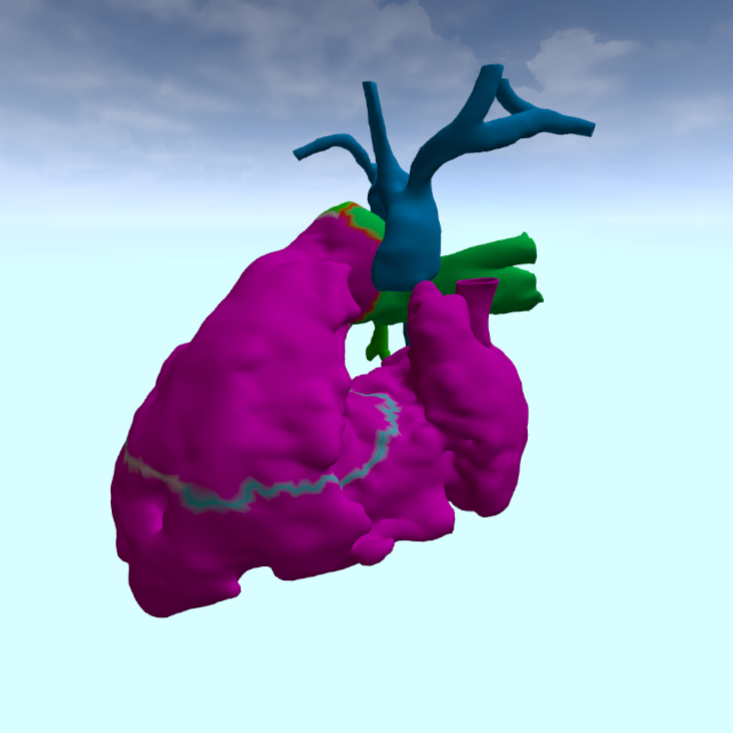
\includegraphics[width=0.7\textwidth]{vrScreenshot/heart.png}
  \caption{3D model of an heart}
  \label{fig:heart}
\end{figure}
\subsection{Existing hardware}

The equipment: The University of Padua has some Meta quest 2 Fig.[\ref{fig:metaQuest2}] a \ac{HMD} for \ac{VR}.\\ 
The Meta Quest 2 is a standalone \ac{HMD}, this means that it doesn't need other peripherals like an external console or \ac{PC} for working.\\
For user interaction, the Meta Quest 2 uses two wireless controllers, but it also has the possibility to use hand-tracking, to let the user navigate the interfaces by using his/her own hands.
The tracking of the user in the real-world environment is achieved using 4 infrared cameras and other sensors like multi axes gyroscopes and accelerometers.\\
They use a custom version of the Android \ac{OS}, this can give a certain degree of liberty in creating APPs for the device.

\begin{figure}[ht]
  \centering
  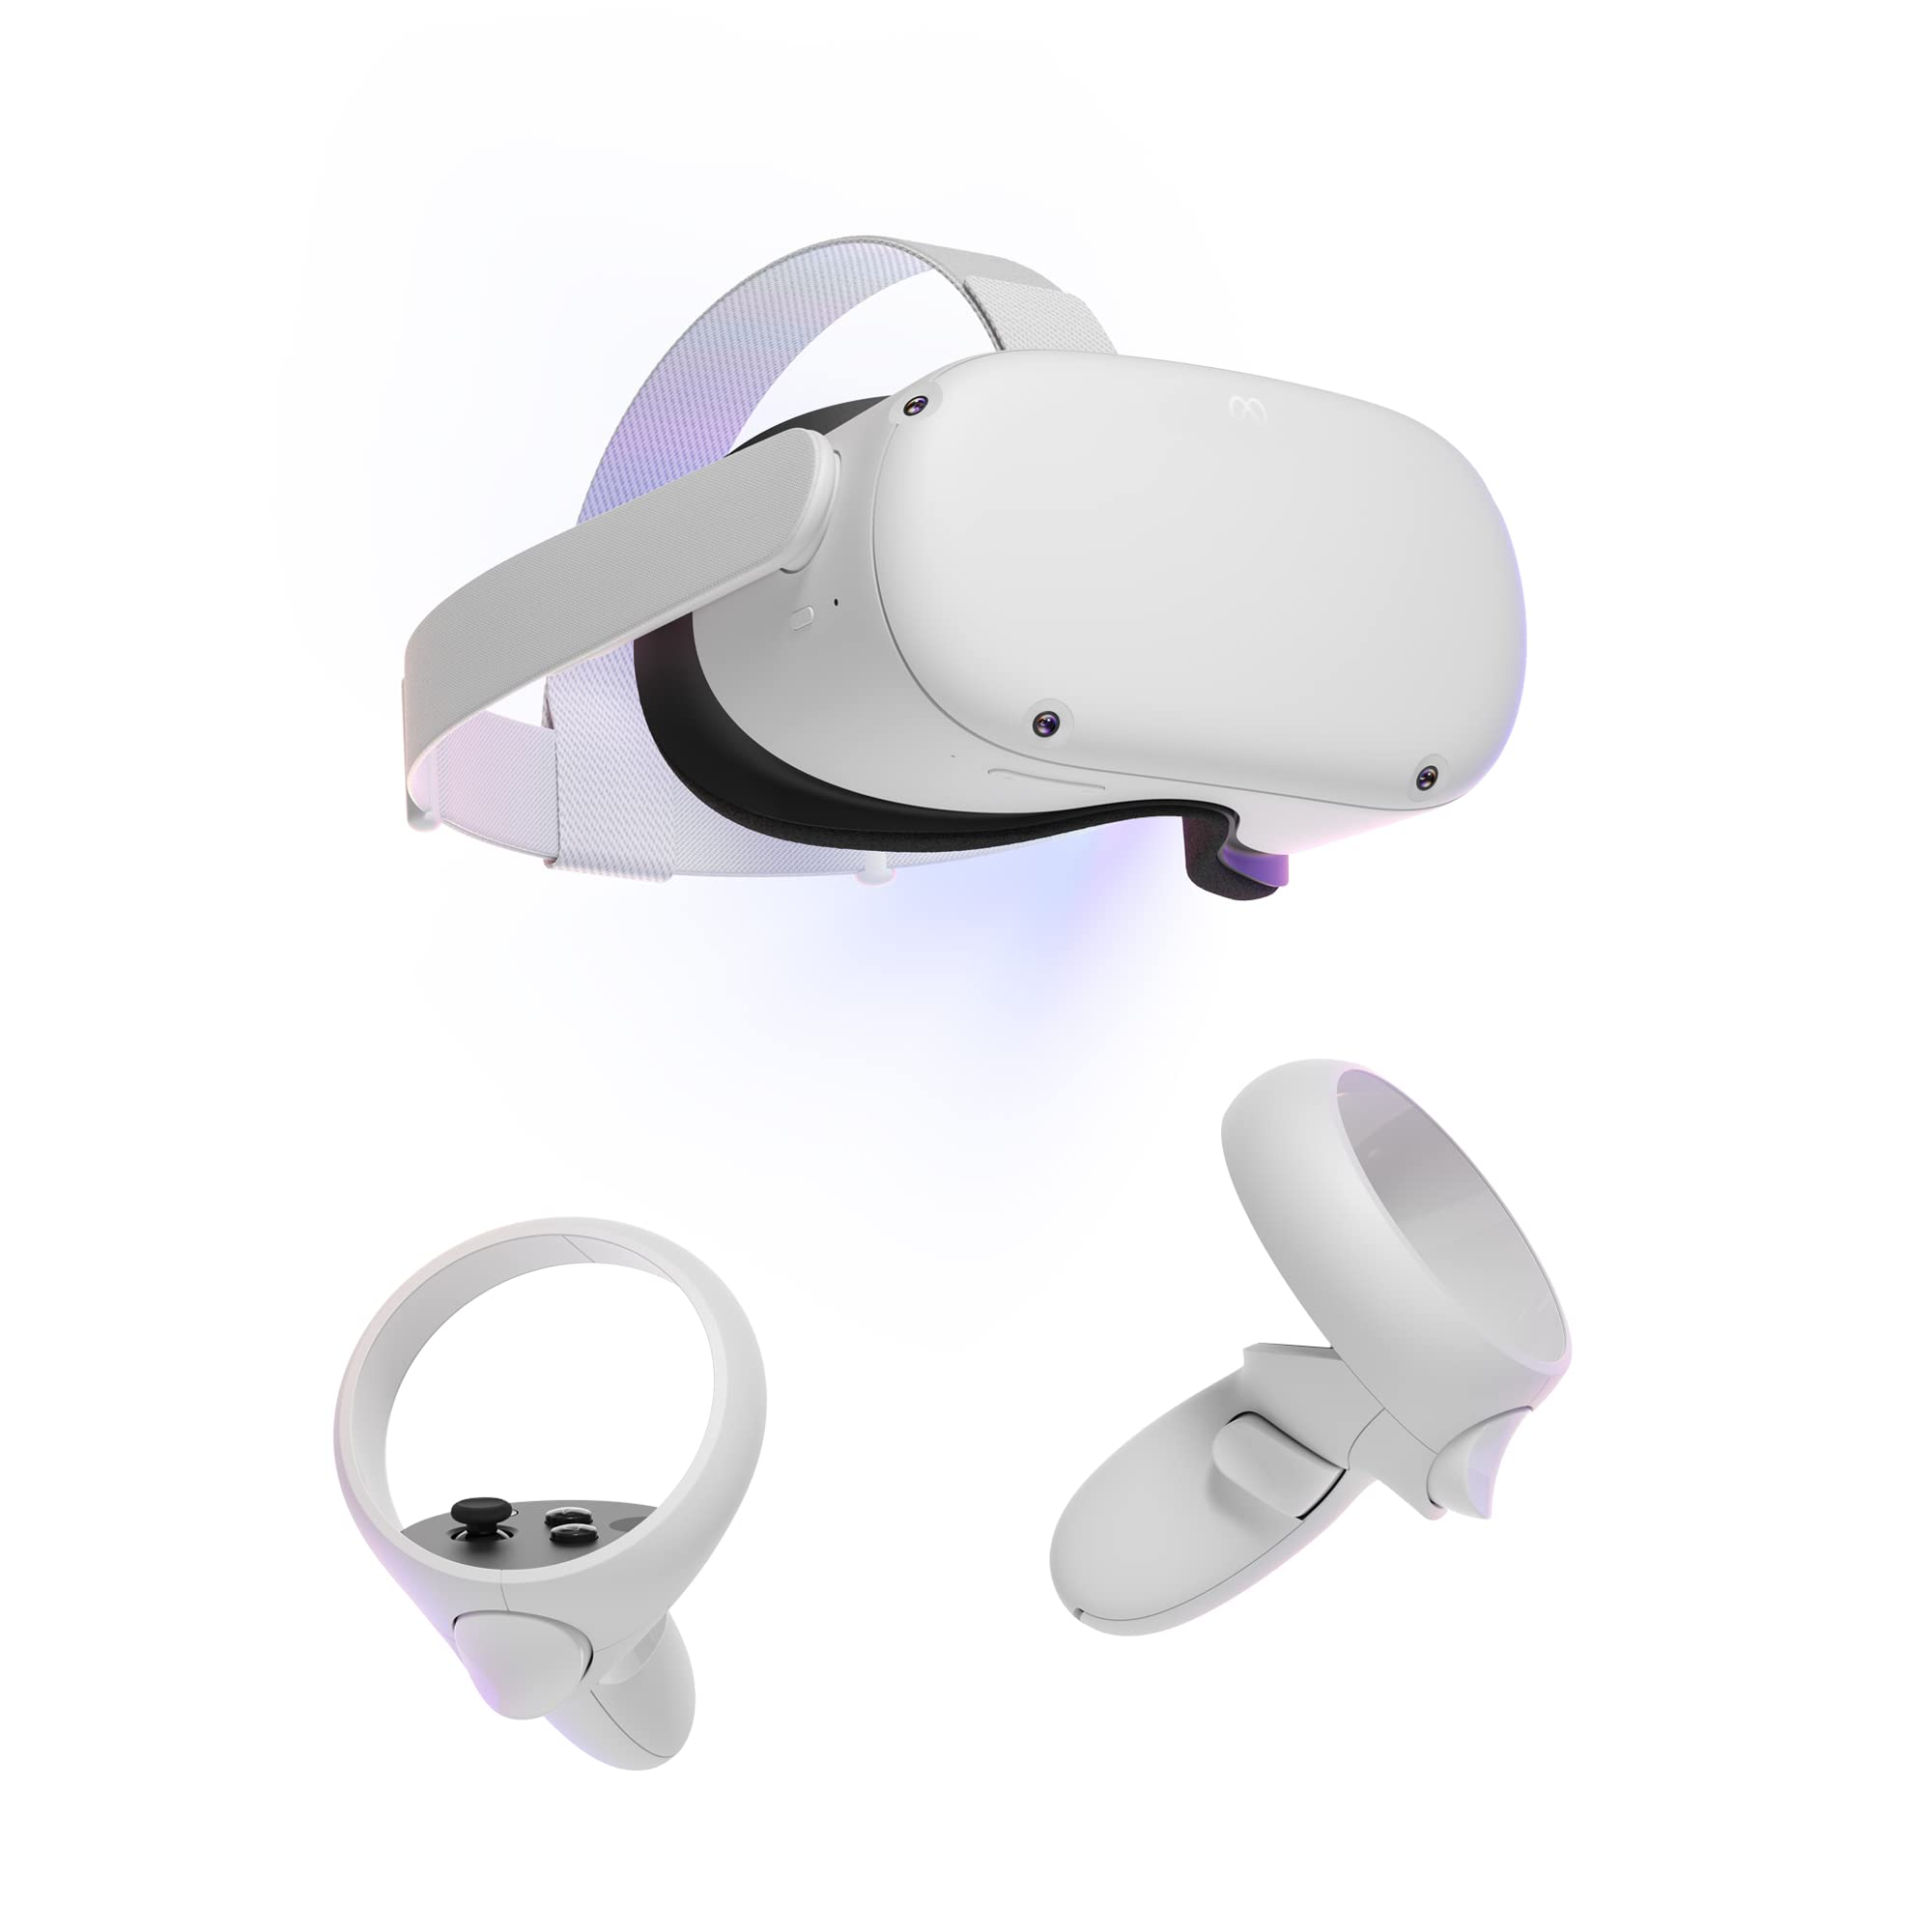
\includegraphics[width=0.5\textwidth]{metaQuest2.jpg}
  \caption{Meta quest 2}
  \label{fig:metaQuest2}
\end{figure}

\paragraph{Use cases of VR:}
Principally the surgeons are using VR equipment for training and showing critical health conditions of different patients' hearts.
They are using an app called Shapes XR, this app has a web app for uploading 3D models and then showing them on the \ac{HMD}.
The app has a multiplayer functionality so that multiple people can look at the 3D models in the environment, even if the developers recommend at max 8 people, they tested with 14 users connected and there weren't any problems.

\subsection{Existing software}

Shapes XR lets you create rooms, accessible via a code, where multiple people can create 3D models with basic tools like 3D brushes and standard shapes like cubes, pyramids and so on.
It also lets you upload a 3D model file on their own website, so that in the home you can download it and start to work on it.
It lets you also create your own avatar.
This is the main feature that the surgeons are using for show the 3D Models

\paragraph{The Problems:}
Unfortunately Shapes XR is principally used for 3D modeling, so the app has a lot of features like changing the scale of the world or brushes for modeling the objects that aren't useful for the surgeons,
and quite distracting because for a lot of people it is the first time using a \ac{HMD}.\\
The user experience is extremely important in \ac{VR} because it is difficult to tutoring the user while using the \ac{HMD}.
Then Shapes XR positions the user in an empty 3D plane with little to none point of reference so If a user accidentally uses the teleport function, they may find themselves somewhere far away from the scene they are supposed to be watching.

\paragraph{Feedbacks from surgeons and nurses:}

There was a lesson on 12/12/2023 with the integration of the Quest 2 and Shapes XR. First it was pretty chaotic, a lot of people did not even know how to use the controllers,
and they had problems even putting in the code for entering the session. Unfortunately we did not have time to make a nice lesson for teaching how to use the HMD,
the tutorial made by Meta approximates takes 15 min to complete, even more if the user wants to try the mini-games, so we did not have the time to show it. The main critical points were: 

\begin{itemize}
  \item Inadequate tutoring for teaching how to use the \ac{HMD}
  \item Difficulty for accessing the multiplayer room
  \item Difficulty at moving in the room
  \item Some people avatar were blocking the visual of some people
\end{itemize}
\noindent
How we can see a new app for this use case could be useful, and this is the main reason why this software exists. 